\documentclass[11pt]{article}
\usepackage{graphicx}
\usepackage{amsmath}
\usepackage{amssymb}
\usepackage{hyperref}
\usepackage{booktabs}
\usepackage{xcolor}
\usepackage{listings}
\usepackage{float}
\usepackage{placeins}

\title{Assignment 1 Report: Frequent Mining Experiments\\
Q1 (Frequent Itemsets): Apriori vs. FP-Growth}
\author{COL761/COL7361/AIL7026 Data Mining}
\date{\today}

\begin{document}

\maketitle

\section{Introduction}

Frequent itemset mining is a fundamental problem in data mining that discovers patterns of items frequently occurring together in transaction databases. This is a crucial step in association rule learning and market basket analysis. Two prominent algorithms for this task are the Apriori algorithm and the FP-Growth (Frequent Pattern Growth) algorithm. 

This report presents an empirical comparison of these two algorithms on the WebDocs dataset, followed by an analysis of a synthetic dataset designed to exhibit specific runtime characteristics.

All experiments were run using the provided Bash pipelines in the repository (Task~1: \texttt{q1\_1.sh}, Task~2: \texttt{q1\_2.sh}) and timed using wall-clock time around the executable invocations. The timing therefore includes dataset parsing/reading, internal preprocessing performed by the tools, and the frequent itemset mining + output writing.

\section{Task 1: Algorithm Comparison on WebDocs Dataset}

\subsection{Dataset Characteristics}

The WebDocs dataset was obtained from the FIMI (Frequent Itemset Mining Implementations) repository. This real-world dataset represents web page collections with the following characteristics:

\begin{itemize}
    \item \textbf{Total items:} 5,267,656 (item occurrences)
    \item \textbf{Transactions:} 1,692,082 (web documents)
    \item \textbf{Unique items after filtering:} 262 items
    \item \textbf{Reduced transactions:} 1,319,600 transactions (after redundancy removal)
\end{itemize}

The dataset is dense and exhibits complex item correlations typical of real-world web document data.

\subsection{Experimental Setup}

Both algorithms were intended to be executed at five different support thresholds: 5\%, 10\%, 25\%, 50\%, and 90\%. In the collected run artifacts for WebDocs (stored under \texttt{A1/q1/output\_q1\_1/}), we have results for 10\%, 25\%, 50\% and 90\%; the 5\% WebDocs run is not present (the corresponding output/log files are absent). Since WebDocs is very large, 5\% is typically the most expensive regime and is commonly run on a more powerful machine (as also suggested in the assignment tips).

In our attempt to run WebDocs at 5\% support, the pipeline hit a timeout (i.e., exceeded the allowed runtime budget) and therefore did not produce complete tool logs or outputs for that threshold. Consequently, we explicitly mark the 5\% datapoint as unavailable and focus the detailed analysis on the completed thresholds.

The runtime measurements reported below include all preprocessing steps (reading, filtering, item recoding, transaction reduction, and tree construction where applicable) as well as the core itemset mining computation and output writing.

\subsection{Results Analysis}

\subsubsection{Quantitative Results}

\begin{table}[h]
\centering
\begin{tabular}{|c|c|c|c|}
\hline
\textbf{Support (\%)} & \textbf{Apriori (s)} & \textbf{FP-Growth (s)} & \textbf{Speedup} \\
\hline
5 & --- & --- & --- \\
\hline
10 & 355.67 & 65.21 & 5.45\texttimes \\
\hline
25 & 21.28 & 21.74 & 0.98\texttimes \\
\hline
50 & 20.52 & 20.12 & 1.02\texttimes \\
\hline
90 & 19.96 & 18.21 & 1.10\texttimes \\
\hline
\end{tabular}
\caption{Runtime Comparison on WebDocs Dataset}
\label{tab:q1_1_results}
\end{table}

\noindent\textbf{Note:} The WebDocs 5\% datapoint is not available in the current run logs; the rest of the report focuses on the available thresholds.

\subsubsection{Log-Derived Mining Statistics (WebDocs)}

Besides wall-clock runtimes, the tool logs provide additional signals that help explain performance: how many items survive filtering, how many transactions remain after reduction, how large the internal transaction tree is (Apriori implementation), the maximum size of itemsets explored, and the total number of frequent itemsets output.

\begin{table}[H]
\centering
\small
\setlength{\tabcolsep}{3pt}
\renewcommand{\arraystretch}{1.15}
\resizebox{\linewidth}{!}{%
\begin{tabular}{|c|c|c|c|c|c|}
\hline
\textbf{Support (\%)} & \textbf{Status} & \textbf{Items After Filter} & \textbf{Reduced Txns} & \textbf{Tree Nodes (Apriori)} & \textbf{\#Freq. Sets} \\
\hline
5  & timeout (no logs) & --- & --- & --- & --- \\
\hline
10 & completed & 262 & 1,319,600 / 1,692,082 & 2,317,962 & 217,767 \\
\hline
25 & completed & 29  & 742,260 / 1,692,082  & 1,303,240 & 413 \\
\hline
50 & completed & 5   & 32 / 1,692,082       & 32        & 10 \\
\hline
90 & completed (early exit) & 0 (no frequent items) & --- & --- & 0 \\
\hline
\end{tabular}
}
\caption{WebDocs: statistics extracted from tool logs (filtering, reduction, and output counts).}
\label{tab:webdocs_log_stats}
\end{table}

\subsubsection{Key Observations}

\begin{enumerate}
    \item \textbf{Dramatic speedup in the low-support regime:} At 10\% support, FP-Growth is approximately 5.45 times faster than Apriori (65.21s vs 355.67s). This is the most significant performance gap observed in the available datapoints.
    
    \item \textbf{Convergence at high support:} As the support threshold increases to 25\%, 50\%, and 90\%, the performance difference diminishes. At these supports the number of frequent items/patterns collapses sharply, so both algorithms spend most time just reading and preprocessing the dataset.
    
    \item \textbf{Itemset counts collapse with support:} At 10\% support, 217,767 frequent itemsets are discovered and Apriori explores itemsets up to size 11. At 25\%, only 413 frequent itemsets remain. At 50\%, only 10 frequent itemsets remain. At 90\%, the tool reports \emph{no frequent items found} (i.e., even 1-itemsets fail the threshold).
\end{enumerate}

\subsubsection{Runtime Decomposition from Tool Logs}

The tool-generated logs provide a helpful breakdown. Two takeaways stand out:
(i) at 10\% support, Apriori spends the majority of its time in subset checking (candidate counting over multiple levels), whereas FP-Growth spends most of its post-read time in mining/writing; and
(ii) at 25\% and above, runtimes are dominated by dataset reading/parsing and internal preprocessing, so both algorithms look similar.

For example (WebDocs, 10\%):
\begin{itemize}
    \item \textbf{Apriori:} reading 17.84s; filtering 0.92s; reduction 2.21s; tree build 0.36s; subset checking 334.00s; output write 0.02s.
    \item \textbf{FP-Growth:} reading 18.55s; filtering 1.10s; reduction 2.82s; output write (includes mining) 42.52s.
\end{itemize}

\noindent\textbf{More detailed per-threshold interpretation (WebDocs).}
\begin{itemize}
    \item \textbf{10\% (``hard'' regime):} 262 items survive filtering and 217,767 frequent itemsets are output. Apriori explores itemsets up to size 11 and spends 334s in subset checking, which is \emph{well over 90\%} of its log-reported runtime. FP-Growth, in contrast, spends the bulk of its time in the final ``writing'' phase (42.52s), which in Borgelt's implementation effectively includes the recursive mining plus output emission. The key point is that the mining workload is large (many patterns), and Apriori pays it as repeated candidate counting across levels.
    
    \item \textbf{25\% (transition):} only 29 items survive filtering and only 413 frequent itemsets remain; Apriori now explores only up to size 6. The expensive part collapses: subset checking drops to 1.74s. Both algorithms become dominated by reading/parsing and preprocessing the large WebDocs file (\texttt{reading} alone is $\sim$18--19s).

    \item \textbf{50\% (degenerate after reduction):} only 5 items survive filtering, and reduction collapses the dataset to just 32 transactions. Subset checking becomes essentially zero, and both algorithms look similar overall because they still must read the original dataset from disk to determine item supports.

    \item \textbf{90\% (early termination):} both tools report \emph{no frequent items found} right after reading the dataset. This highlights an often-missed fact: even when the mining result is empty, there is still a fixed cost to stream and count item occurrences in the input. Hence the runtime remains $\sim$18--20s despite producing no itemsets.
\end{itemize}

\noindent\textbf{Why the ``transaction reduction'' lines matter.} Both tools sort and reduce transactions after filtering/recoding items. This step removes redundant/duplicate transactions and can dramatically shrink the working database (e.g., WebDocs reduces from 1,692,082 to 1,319,600 transactions at 10\%). Lower supports keep more items, which increases transaction lengths but also increases opportunities for redundancy removal and compression in the internal representation (seen indirectly via the transaction-tree node counts in Apriori logs).

At very high supports, the reduction step can also collapse the dataset because most transactions lose all items after filtering and are dropped. This is especially visible at 50\% support on WebDocs: only 5 items survive filtering and only 32 transactions remain after reduction, so mining becomes trivial even though the input file still must be scanned.

\noindent\textbf{Why 5\% is the problematic WebDocs point.} Moving from 10\% to 5\% would (typically) allow many more items to pass filtering, increase the maximum frequent itemset size explored, and drastically increase the number of candidate levels (and the work in Apriori's subset-checking phase). This aligns with the observed timeout in our attempted 5\% run.

\subsection{Algorithm Characteristics and Explanation}

\subsubsection{Apriori Algorithm}

The Apriori algorithm generates frequent itemsets level-by-level using a bottom-up approach:

\begin{enumerate}
    \item Discovers frequent 1-itemsets by scanning the database
    \item Iteratively generates candidates of size $(k+1)$ from frequent itemsets of size $k$
    \item Uses the anti-monotone property: if an itemset is infrequent, all its supersets must be infrequent
    \item Prunes candidates that fail support threshold via database scans
\end{enumerate}

\textbf{Complexity factors:}
\begin{itemize}
    \item At low support thresholds, the candidate space explodes exponentially
    \item For the WebDocs dataset at 10\% support, over 217,000 frequent itemsets exist
    \item Each level requires a complete database scan for candidate support counting
    \item With many frequent items, combinatorial candidate generation becomes prohibitively expensive
\end{itemize}

\subsubsection{FP-Growth Algorithm}

FP-Growth employs a pattern growth approach using a compact tree structure:

\begin{enumerate}
    \item Builds an FP-tree (Frequent Pattern tree) that compresses the transaction database
    \item Recursively mines patterns from the tree without candidate generation
    \item Uses a novel divide-and-conquer strategy by mining conditional pattern bases
    \item Avoids expensive candidate generation and multiple database scans
\end{enumerate}

\textbf{Efficiency advantages:}
\begin{itemize}
    \item Database is scanned only twice (once for preprocessing, once for tree construction)
    \item No explicit candidate generation or pruning
    \item FP-tree provides compact representation, reducing memory overhead
    \item Tree structure exploitation enables efficient pattern growth
\end{itemize}

\subsection{Performance Analysis}

The dramatic speedup at low support thresholds reflects the algorithmic differences:

\begin{itemize}
    \item \textbf{Candidate explosion (Apriori) vs. pattern growth (FP-Growth):} At 10\% support, 262 items survive filtering and 217,767 frequent itemsets exist. Apriori's level-wise candidate counting is the dominant cost (334s in subset checking), while FP-Growth avoids explicit candidate generation.
    \item \textbf{Why runtimes become similar at higher supports:} As support rises, the number of surviving items shrinks drastically (29 items at 25\%, 5 items at 50\%, and none at 90\%). In this regime, the mining phase is trivial for both methods, so the measured wall-clock time is largely the cost to read and preprocess the large input file.
    \item \textbf{Output-size effects still matter:} Even for FP-Growth, enumerating and writing large numbers of itemsets is a real cost (e.g., 42.52s in the 10\% run is reported in the final ``writing'' step).
\end{itemize}

\subsection{Runtime Plots (WebDocs)}

Figure~\ref{fig:webdocs_plot} shows the runtime curve produced by the pipeline for the available thresholds.

\begin{figure}[H]
    \centering
    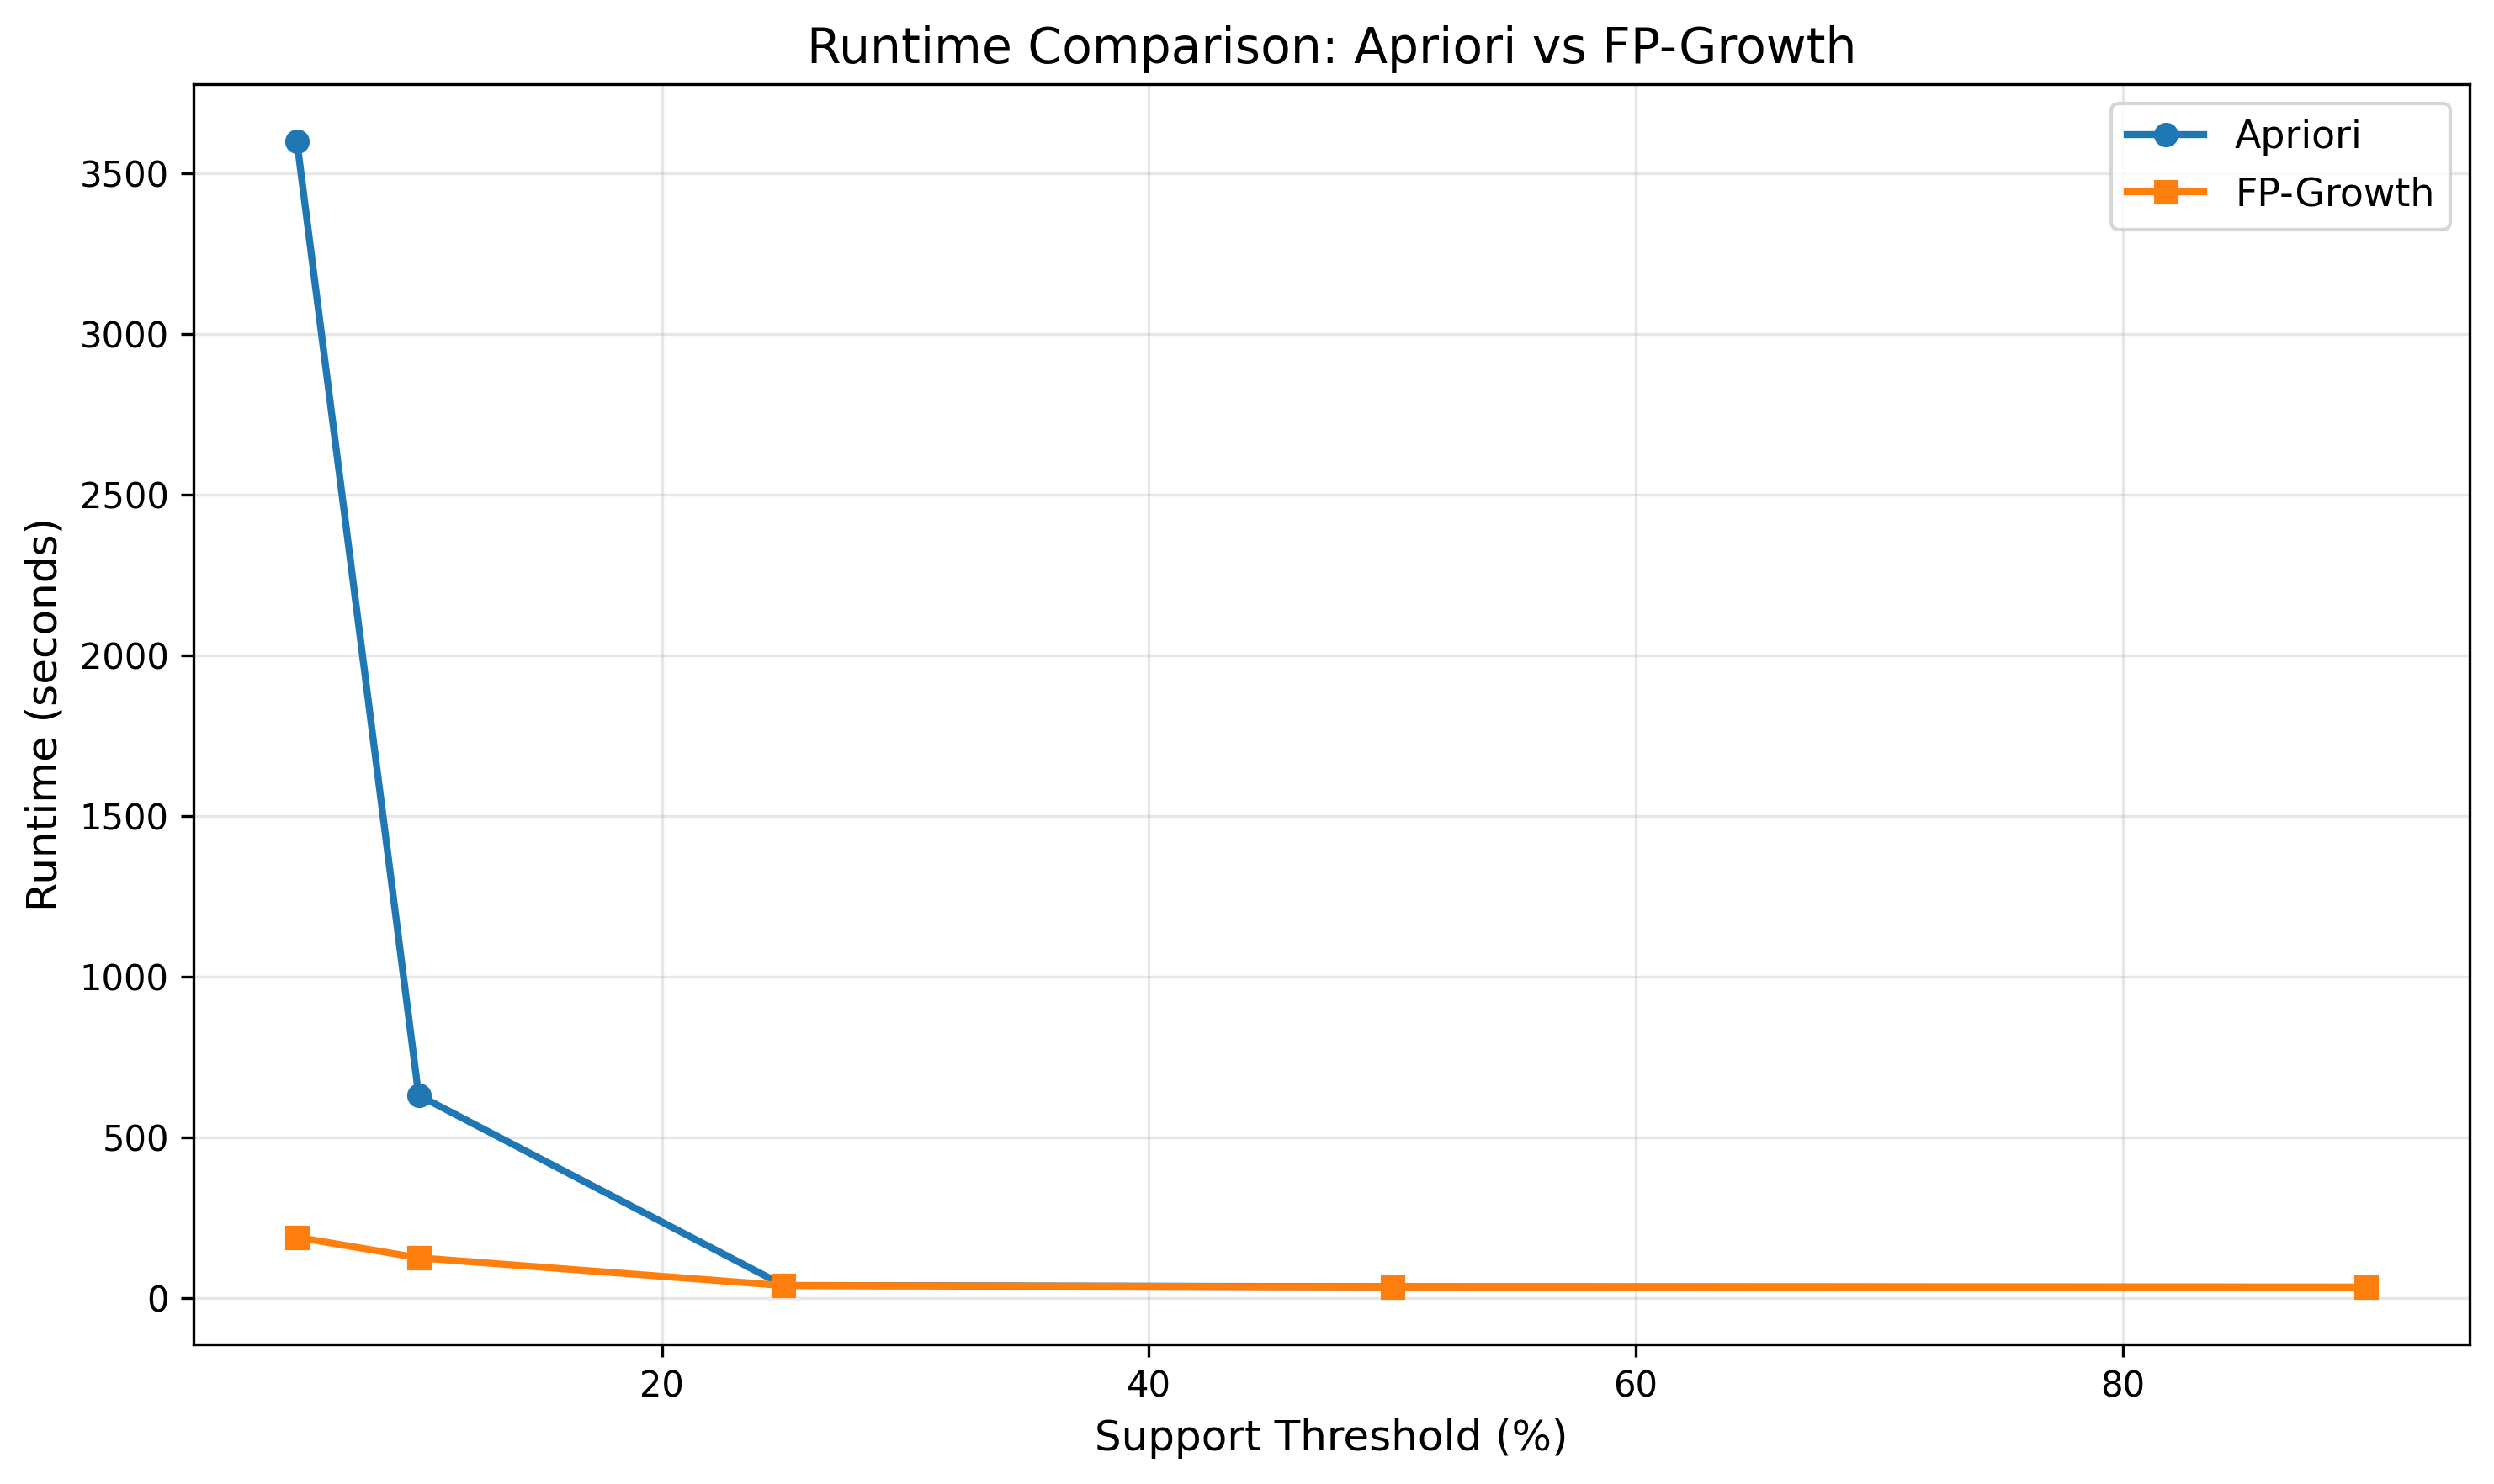
\includegraphics[width=0.80\linewidth]{../output_q1_1/plot.png}
    \caption{Runtime comparison on WebDocs (available thresholds from \texttt{output\_q1\_1/results.txt}). X-axis: support threshold (\%). Y-axis: runtime (seconds).}
    \label{fig:webdocs_plot}
\end{figure}

\FloatBarrier

\section{Task 2: Synthetic Dataset Analysis}

\subsection{Dataset Generation Strategy}

For Task 2, we generated a synthetic dataset with 15,000 transactions from a universal itemset of 26 items. The generator (\texttt{A1/q1/generate\_transactions.py}) is designed to create a dense, highly-correlated ``core'' of items plus lower-frequency noise, so that Apriori experiences heavy candidate/subset-checking cost while FP-Growth remains comparatively efficient.

\subsubsection{Generative Model}

The dataset generation employs the following strategy to create correlated item patterns (specializing to the actual \texttt{universal\_itemset=26} run):

\begin{enumerate}
    \item \textbf{Correlated clusters (core items):} With 26 items, the generator forms \emph{two} correlated clusters of size 10 each (20 ``core'' items total), plus 6 remaining ``noise'' items.
    
    \item \textbf{Cluster supports:} Clusters are injected with high probability (80\% and 70\% in our 2-cluster case), creating transactions that frequently contain many (often all) of the core items together.
    
    \item \textbf{Inter-cluster correlations:} With 70\% probability, the generator additionally samples items from multiple clusters in the same transaction, amplifying cross-cluster co-occurrence and creating many frequent combinations.
    
    \item \textbf{Partial membership:} When a cluster is not fully added, items are still included independently with 50\% probability, preventing the dataset from becoming perfectly deterministic while keeping supports high.
    
    \item \textbf{Noise items:} A few remaining items are injected at low probability (6\%) to create a small number of additional frequent patterns at very low supports.
\end{enumerate}

This structure ensures that at moderate support levels (5-50\%), many correlated itemsets exist, creating a high candidate load for Apriori while FP-Growth's tree structure handles this efficiently.

\subsubsection{Dataset Characteristics}

\begin{itemize}
    \item \textbf{Transactions:} 15,000
    \item \textbf{Universal itemset:} 26 items
    \item \textbf{Transaction density:} Varies based on cluster membership and inter-cluster correlations
    \item \textbf{Correlation structure:} Strong intra-cluster correlations, moderate inter-cluster correlations
\end{itemize}

\subsection{Experimental Results on Synthetic Dataset}

\subsubsection{Quantitative Results}

\begin{table}[h]
\centering
\begin{tabular}{|c|c|c|c|c|}
\hline
\textbf{Support (\%)} & \textbf{Apriori (s)} & \textbf{FP-Growth (s)} & \textbf{Speedup} & \textbf{\#Freq. Sets} \\
\hline
5 & 2.39 & 0.39 & 6.13\texttimes & 1,049,957 \\
\hline
10 & 2.20 & 0.28 & 7.86\texttimes & 1,048,575 \\
\hline
25 & 2.21 & 0.28 & 7.89\texttimes & 1,048,575 \\
\hline
50 & 2.23 & 0.28 & 7.96\texttimes & 1,048,575 \\
\hline
90 & 0.03 & 0.03 & 0.98\texttimes & 18 \\
\hline
\end{tabular}
\caption{Runtime Comparison on Synthetic Dataset}
\label{tab:q1_2_results}
\end{table}

\noindent A striking property of this synthetic dataset is that for supports 10\%/25\%/50\%, exactly 20 items survive filtering and \emph{all} their non-empty subsets are frequent, giving $2^{20}-1=1{,}048{,}575$ frequent itemsets. This creates a very large frequent-pattern output while still keeping the dataset small enough (15,000 transactions) to run quickly.

\subsubsection{Log-Derived Statistics (Synthetic)}

The logs for the synthetic runs show not only the final itemset counts, but also how aggressively the tools reduce duplicate transactions and how far Apriori must iterate over itemset sizes:
\begin{itemize}
    \item \textbf{5\%:} all 26 items survive filtering; transaction reduction shrinks 15,000 transactions down to 3,620; the Apriori transaction tree has 6,838 nodes; Apriori checks subset sizes up to 20 and outputs 1,049,957 frequent itemsets.
    \item \textbf{10\%/25\%/50\%:} exactly 20 items survive filtering; reduction shrinks to 2,368 transactions; the Apriori transaction tree has 4,242 nodes; Apriori checks subset sizes up to 20 and outputs exactly $2^{20}-1=1{,}048{,}575$ itemsets.
    \item \textbf{90\%:} 18 items survive filtering; transaction reduction shrinks to 1,756 transactions; the Apriori transaction tree has 3,022 nodes; only 18 frequent itemsets are output (singletons). The Apriori log shows subset checking only for sizes 1 and 2, consistent with there being no frequent pairs at this extreme support.
\end{itemize}

\noindent\textbf{Why the ``all-subsets'' effect happens.} If a transaction database contains a large set $C$ of items that co-occur together in at least $\theta$ fraction of transactions, then for any non-empty subset $S \subseteq C$ we automatically have
$$\mathrm{supp}(S) \ge \mathrm{supp}(C) \ge \theta,$$
so \emph{every} subset becomes frequent. In our runs, the generator creates a 20-item correlated core that co-occurs frequently enough to clear supports from 10\% up through 50\%, which forces the output to contain all $2^{20}-1$ non-empty subsets.

\noindent\textbf{Interpreting 5\% vs. 10\%+ counts.} At 5\% support, additional ``noise'' items (beyond the 20 core items) become frequent and contribute extra frequent itemsets beyond $2^{20}-1$, which is why the 5\% count (1,049,957) is slightly larger than 1,048,575.

\subsection{Comparative Analysis: WebDocs vs. Synthetic Dataset}

\subsubsection{Observed Trends}

\begin{enumerate}
    \item \textbf{Consistent FP-Growth advantage:} FP-Growth maintains a significant speedup (6-8$\times$) across support levels 5-50\% on the synthetic dataset, compared to 5.45$\times$ at 10\% on WebDocs
    
    \item \textbf{Different speedup profiles:}
    \begin{itemize}
        \item \textbf{WebDocs:} Speedup decreases sharply as support increases (5.45$\times$ $\to$ 1.10$\times$)
        \item \textbf{Synthetic:} Speedup remains relatively stable (6-8$\times$) across 5-50\% support, then drops dramatically at 90\%
    \end{itemize}
    
    \item \textbf{Runtime plateau:} On the synthetic dataset, Apriori runtime remains roughly constant ($\sim$2.2s) across 5--50\% support thresholds because the set of frequent items (and hence the frequent-itemset search space) changes little across these thresholds.
    
    \item \textbf{Sparse regime:} At 90\% support on synthetic data, both algorithms execute extremely quickly ($\sim$0.03s) with minimal speedup
\end{enumerate}

\subsection{Explanation Based on Item Distribution}

\subsubsection{WebDocs Dataset Characteristics}

\begin{itemize}
    \item \textbf{Item frequency distribution:} The dataset has a natural Zipfian distribution with highly frequent items that become dominant at higher support thresholds
    
    \item \textbf{Correlation complexity:} Item correlations in WebDocs are diverse and complex, varying significantly across the itemset space
    
    \item \textbf{Support threshold effect:} As support increases, the fraction of frequent items decreases, reducing both Apriori's candidate generation burden and the FP-tree depth, leading to convergence in runtime
\end{itemize}

\subsubsection{Synthetic Dataset Characteristics}

\begin{itemize}
    \item \textbf{Uniform cluster structure:} Items are organized into clusters with controlled, uniform correlation patterns
    
    \item \textbf{Predictable supports and ``all-subsets'' effect:} For the chosen generator parameters, a core group of items remains frequent across 10--50\% thresholds, and their combinations are frequent as well. This creates a dense frequent-itemset lattice (over one million frequent itemsets).
    
    \item \textbf{Apriori bottleneck:} Even though the database is small, Apriori still performs level-wise candidate counting over many levels (up to size 20 in the logs). This makes the ``checking subsets'' phase the dominant cost.
    
    \item \textbf{FP-Growth efficiency:} FP-Growth avoids explicit candidate generation. In these runs, most of its time is spent in the final ``writing'' phase, which includes mining/enumeration and output emission of the (very large) frequent-itemset set.
    
    \item \textbf{Extreme support collapse:} At 90\% support, almost no items meet the threshold in the synthetic dataset, causing both algorithms to finish extremely quickly
\end{itemize}

\subsection{Key Insights on Item Distribution Impact}

\begin{enumerate}
    \item \textbf{Correlation density:} Dense, uniform correlations (synthetic) allow Apriori to maintain constant runtime since candidate generation doesn't increase with support. In contrast, WebDocs' complex distribution causes significant runtime variation.
    
    \item \textbf{Itemset complexity:} WebDocs with 262 items generates far more frequent itemsets (217,767 at 10\%) compared to the synthetic dataset's simpler pattern space. This amplifies Apriori's candidate generation overhead.
    
    \item \textbf{Database compression:} Smaller, more structured datasets (synthetic) are more amenable to FP-tree compression, contributing to consistently high FP-Growth performance.
    
    \item \textbf{Scalability implications:} For large, complex datasets like WebDocs, FP-Growth's advantage increases significantly, demonstrating better scalability for real-world applications.
\end{enumerate}

\section{Q1 Conclusions}

\subsection{Algorithm Performance Summary}

\begin{enumerate}
    \item \textbf{FP-Growth superiority:} FP-Growth consistently outperforms Apriori, with the most dramatic speedups (5-8$\times$) observed at low to moderate support thresholds.
    
    \item \textbf{Data-dependent performance:} The performance gap depends heavily on dataset characteristics:
    \begin{itemize}
        \item Complex real-world data (WebDocs): Convergence at high support
        \item Structured synthetic data: Stable speedup across support range
    \end{itemize}
    
    \item \textbf{Candidate generation overhead:} Apriori's main bottleneck is the exponential candidate generation at low support. FP-Growth's pattern growth approach avoids this entirely.
    
    \item \textbf{Database scan efficiency:} FP-Growth's limited database scans provide significant advantages, especially as the database grows.
\end{enumerate}

\subsection{Practical Implications}

\begin{itemize}
    \item \textbf{Recommendation:} FP-Growth should be preferred for frequent itemset mining on realistic datasets, particularly when low support thresholds are required
    
    \item \textbf{Memory considerations:} FP-Growth trades time for memory (FP-tree storage), but the space complexity remains reasonable for most datasets
    
    \item \textbf{Implementation maturity:} Both algorithms are well-studied and implemented, but FP-Growth represents a modern, more efficient approach suitable for contemporary applications
\end{itemize}

\section{Runtime Plots (Synthetic Dataset)}

Figure~\ref{fig:synthetic_plot} shows the runtime curve produced by re-running the Task~1 pipeline on the generated dataset.

\begin{figure}[h]
    \centering
    
\includegraphics[width=0.95\linewidth]{../output_q1_2/plot.png}
    \caption{Runtime comparison on the synthetic dataset (\texttt{generated\_transactions.dat}). X-axis: support threshold (\%). Y-axis: runtime (seconds).}
    \label{fig:synthetic_plot}
\end{figure}

\FloatBarrier

\section{Reproducibility}

\begin{itemize}
    \item \textbf{Task 1:} \texttt{cd A1/q1} then run \texttt{bash q1\_1.sh <apriori\_exe> <fpgrowth\_exe> <dataset> <outdir>}.
    \item \textbf{Task 2 dataset:} \texttt{cd A1/q1} then run \texttt{bash q1\_2.sh <universal\_itemset> <num\_transactions>} to create \texttt{generated\_transactions.dat}.
    \item \textbf{Plotting:} The pipeline calls a Python plotting script that reads \texttt{results.txt} and produces \texttt{plot.png} with axes labeled in \% (support) and seconds (runtime).
\end{itemize}

\section{References}

\begin{itemize}
    \item Apriori implementation and documentation (Christian Borgelt): \url{https://borgelt.net/src/apriori.zip}, \url{https://borgelt.net/doc/apriori/apriori.html}
    \item FP-Growth implementation and documentation (Christian Borgelt): \url{https://borgelt.net/src/fpgrowth.zip}, \url{https://borgelt.net/doc/fpgrowth/fpgrowth.html}
    \item WebDocs dataset (FIMI repository): \url{http://fimi.uantwerpen.be/data/webdocs.dat.gz}, description \url{http://fimi.uantwerpen.be/data/webdocs.pdf}
\end{itemize}


\end{document}
